\documentclass[11pt,aspectratio=169]{beamer}

\usetheme{Madrid}
\usecolortheme{seahorse}

\usepackage[utf8]{inputenc}
\usepackage{amsmath,amssymb}
\usepackage{algpseudocode}
\usepackage{algorithmicx}
\usepackage{xcolor}
\usepackage{listings}
\usepackage{booktabs}
\usepackage{tikz}
\usetikzlibrary{arrows.meta,positioning,fit,backgrounds}

\setbeamertemplate{navigation symbols}{}
\setbeamertemplate{footline}[frame number]

\lstdefinestyle{py}{
  language=Python,
  basicstyle=\ttfamily\scriptsize,
  keywordstyle=\color{blue!70!black}\bfseries,
  commentstyle=\color{gray},
  stringstyle=\color{green!40!black},
  showstringspaces=false,
  breaklines=true,
  numbers=left,
  numberstyle=\tiny\color{gray},
  frame=single,
  xleftmargin=1.5em,
  aboveskip=0.3em,
  belowskip=0.3em
}

\title{LeetCode Deep Dive}
\subtitle{From First Instinct to Optimal Algorithm: MST and Minimax Paths in Practice\\
\small Week 5 Supplement -- TOAE209/TOAH209: Design and Analysis of Algorithms}
\author{Foreign Trade University}
\date{}

\begin{document}

\begin{frame}
  \titlepage
\end{frame}

\begin{frame}{Outline}
  \tableofcontents
\end{frame}

% =================================================================
\section{Problem 1 (Medium): Min Cost to Connect All Points}
% =================================================================

\begin{frame}{Problem statement}
  \begin{block}{LeetCode 1584 -- Min Cost to Connect All Points (\textcolor{blue!50!black}{Medium})}
    Given $n$ points on a 2D plane, the cost to connect two points is their
    \textbf{Manhattan distance} $|x_i-x_j|+|y_i-y_j|$. Connect \emph{all} points
    so that there is exactly one path between any two of them, minimizing total
    cost. Return the minimum total cost.
  \end{block}
  \begin{itemize}
    \item Constraints (LeetCode): $1 \le n \le 1000$.
    \item ``Exactly one path between any two points'' is the definition of a
    \textbf{spanning tree}. Minimizing its total edge weight is exactly this
    week's \textbf{minimum spanning tree} problem, on the \emph{complete} graph
    where every pair of points is an edge.
  \end{itemize}
\end{frame}

\begin{frame}{Worked example}
  \begin{columns}
  \begin{column}{0.46\textwidth}
  \begin{center}
  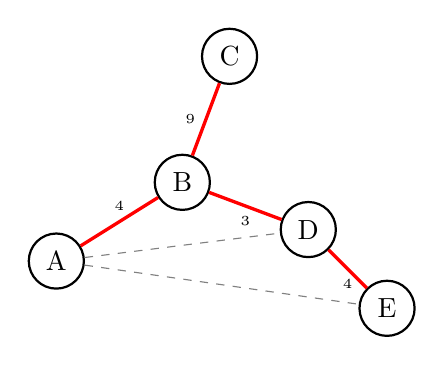
\begin{tikzpicture}[vtx/.style={circle, draw, thick, minimum size=7mm}, >=Stealth]
    \node[vtx] (A) at (0,0)     {A};
    \node[vtx] (B) at (1.6,1.0) {B};
    \node[vtx] (C) at (2.2,2.6) {C};
    \node[vtx] (D) at (3.2,0.4) {D};
    \node[vtx] (E) at (4.2,-0.6){E};
    \draw[very thick, red]  (B)--(D) node[midway,below,font=\tiny,black]{3};
    \draw[very thick, red]  (A)--(B) node[midway,above,font=\tiny,black]{4};
    \draw[very thick, red]  (D)--(E) node[midway,below,font=\tiny,black]{4};
    \draw[very thick, red]  (B)--(C) node[midway,left,font=\tiny,black]{9};
    \draw[dashed, gray] (A)--(D);
    \draw[dashed, gray] (A)--(E);
  \end{tikzpicture}
  \end{center}
  \end{column}
  \begin{column}{0.54\textwidth}
  \scriptsize
  $A(0,0)$, $B(2,2)$, $C(3,10)$, $D(5,2)$, $E(7,0)$ (not to scale).
  \begin{itemize}
    \item All $\binom{5}{2}=10$ pairwise Manhattan distances exist as candidate
    edges (dashed = a sample of the ones \emph{not} used).
    \item MST (red): $BD{=}3$, $AB{=}4$, $DE{=}4$, $BC{=}9$.
    \item \textbf{Answer: $3+4+4+9=20$.}
  \end{itemize}
  \end{column}
  \end{columns}
\end{frame}

\begin{frame}{First instinct: enumerate spanning trees}
  \begin{block}{Most direct reading of the problem}
    ``Find the cheapest way to connect all points into a tree'' $\Rightarrow$
    enumerate every possible spanning tree on the $n$ points, compute its total
    cost, keep the cheapest.
  \end{block}
  \begin{itemize}
    \item By Cayley's formula, a complete graph on $n$ labeled vertices has
    $n^{n-2}$ distinct spanning trees.
    \item For $n=10$: $10^8$ trees. For $n=1000$ (this problem's actual limit):
    $1000^{998}$ -- a number with about 3000 digits. There is no computer, now
    or ever, that enumerates this.
  \end{itemize}
\end{frame}

\begin{frame}{The structural insight}
  \begin{itemize}
    \item This is \emph{exactly} the MST problem from this week's lecture, on
    the complete graph where every pair of points is an edge with weight equal
    to their Manhattan distance.
    \item The \textbf{cut property} says: for any partition of the points into
    two groups, the cheapest edge crossing that partition is safe to add. Greedy
    algorithms (Kruskal, Prim) exploit this \emph{locally}, one cut at a time --
    no enumeration of trees is ever needed.
    \item The only remaining question is which greedy algorithm to run --
    and here the graph's \textbf{density} matters.
  \end{itemize}
\end{frame}

\begin{frame}{Choosing Kruskal vs.\ Prim: density matters}
  \begin{itemize}
    \item The graph is \textbf{complete}: $m = \binom{n}{2} = \Theta(n^2)$ edges.
    \item \textbf{Kruskal} needs to generate and sort all $\Theta(n^2)$ edges
    first: $O(n^2\log n)$, then Union-Find in $O(n^2\,\alpha(n))$ -- dominated by
    the sort.
    \item \textbf{Prim with a binary heap} is $O((m+n)\log n) = O(n^2\log n)$ --
    the heap does not help here, because $m=\Theta(n^2)$ already dominates.
    \item \textbf{Prim with a plain array} (no heap: scan all unvisited vertices
    for the minimum each round) is $O(n^2)$ -- strictly better, because it never
    needs to build or sort an edge list at all.
  \end{itemize}
  \begin{alertblock}{The implementation-choice lesson}
    ``Use a heap'' is not always the optimal move -- on a \emph{dense} graph,
    array-based Prim beats both Kruskal and heap-based Prim.
  \end{alertblock}
\end{frame}

\begin{frame}{Optimal algorithm: array-based Prim}
  \footnotesize
  \begin{algorithmic}[1]
    \Function{MinCostConnect}{points}
      \State $dist[0] \gets 0$; $dist[i] \gets \infty$ for $i>0$; $visited \gets \emptyset$; $total \gets 0$
      \For{$n$ rounds}
        \State $u \gets \arg\min_{i \notin visited} dist[i]$ \Comment{scan all unvisited, $O(n)$}
        \State $visited \gets visited \cup \{u\}$;\ $total \gets total + dist[u]$
        \For{each $v \notin visited$}
          \State $dist[v] \gets \min(dist[v],\ \textsc{ManhattanDist}(u,v))$
        \EndFor
      \EndFor
      \State \Return $total$
    \EndFunction
  \end{algorithmic}
  $n$ rounds $\times$ $O(n)$ work per round (scan + relax) $= O(n^2)$ total --
  the same ``relax a distance array'' idea as Dijkstra, from earlier this week.
\end{frame}

\begin{frame}{Trace on the worked example}
  \scriptsize
  Start at $A$. $dist[\cdot]$ shown after each round's relaxation.
  \begin{center}
  \begin{tabular}{@{}c c c c c c c@{}}
    \toprule
    round & pick & cost added & running total & $dist[B]$ & $dist[D]$ & $dist[E]$ \\
    \midrule
    1 & $A$ & 0 & 0 & 4 & 7 & 7 \\
    2 & $B$ & 4 & 4 & -- & 3 & 7 \\
    3 & $D$ & 3 & 7 & -- & -- & 4 \\
    4 & $E$ & 4 & 11 & -- & -- & -- \\
    5 & $C$ & 9 & 20 & -- & -- & -- \\
    \bottomrule
  \end{tabular}
  \end{center}
  ($dist[C]$ column omitted for space: it settles at $13\to9\to9\to9\to9$, picked
  last.) Total $=20$, matching Kruskal's answer from the diagram two slides ago
  -- confirming MST weight is independent of which correct algorithm computes it.
\end{frame}

\begin{frame}{Complexity: three approaches}
  \begin{center}
  \begin{tabular}{@{}lll@{}}
    \toprule
    Approach & Time & Note \\
    \midrule
    Enumerate all spanning trees & $O(n^{n-2})$ & never finishes for $n>{\sim}10$ \\
    Kruskal (sort $\Theta(n^2)$ edges) & $O(n^2\log n)$ & correct, not the fastest here \\
    \textbf{Prim, array-based} & $\boldsymbol{O(n^2)}$ & optimal for this dense graph \\
    \bottomrule
  \end{tabular}
  \end{center}
\end{frame}

\begin{frame}[fragile]{Python implementation}
  \begin{lstlisting}[style=py,aboveskip=0pt,belowskip=0pt]
def minCostConnectPoints(points):
    n = len(points)
    visited = [False] * n
    dist = [float('inf')] * n
    dist[0] = 0
    total = 0

    for _ in range(n):
        u = min((d, i) for i, d in enumerate(dist) if not visited[i])[1]
        visited[u] = True
        total += dist[u]
        xu, yu = points[u]
        for v in range(n):
            if not visited[v]:
                xv, yv = points[v]
                manhattan = abs(xu - xv) + abs(yu - yv)
                if manhattan < dist[v]:
                    dist[v] = manhattan
    return total
  \end{lstlisting}
\end{frame}

\begin{frame}{Implementation tips \& tricks (the programming side)}
  \small
  \begin{itemize}
    \item \textbf{Don't build an adjacency list or edge list at all.} Since the
    graph is complete, Manhattan distance is computed \emph{on the fly} from the
    two points' coordinates -- storing $\Theta(n^2)$ edges explicitly would waste
    memory and time that array-based Prim never needs.
    \item \textbf{The unvisited-minimum scan, not a heap, is the right tool
    here.} \texttt{min((d, i) for i, d in enumerate(dist) if not visited[i])} is
    a plain $O(n)$ scan; pushing every relaxed distance into a \texttt{heapq}
    instead would add $O(\log n)$ per operation for no asymptotic benefit on a
    dense graph, while also needing ``lazy deletion'' of stale heap entries.
    \item \textbf{Unpack coordinates once per outer iteration}
    (\texttt{xu, yu = points[u]}), not once per inner-loop comparison -- a small
    but real constant-factor saving repeated $n$ times per round.
  \end{itemize}
\end{frame}

% =================================================================
\section{Problem 2 (Hard): Swim in Rising Water}
% =================================================================

\begin{frame}{Problem statement}
  \begin{block}{LeetCode 778 -- Swim in Rising Water (\textcolor{red!60!black}{Hard})}
    An $n\times n$ grid has elevation $grid[i][j]$ at cell $(i,j)$. At time $t$
    the water level is $t$; you may move between two \textbf{adjacent} cells
    only if \emph{both} have elevation $\le t$. Starting at $(0,0)$ at time $0$,
    find the minimum $t$ at which $(n-1,n-1)$ is reachable.
  \end{block}
  \begin{itemize}
    \item Constraints (LeetCode): $1 \le n \le 50$, elevations are a permutation
    of $0,\dots,n^2-1$.
    \item Reframe: you need the path from $(0,0)$ to $(n{-}1,n{-}1)$ that
    minimizes its \textbf{maximum} elevation -- a \textbf{minimax path}, not a
    shortest (minimum-\emph{sum}) path.
  \end{itemize}
\end{frame}

\begin{frame}{Worked example}
  \begin{columns}
  \begin{column}{0.46\textwidth}
  \begin{center}
  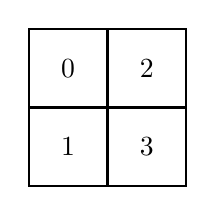
\begin{tikzpicture}[cell/.style={draw, thick, minimum size=10mm}, >=Stealth]
    \node[cell] (a) at (0,1) {0};
    \node[cell] (b) at (1,1) {2};
    \node[cell] (c) at (0,0) {1};
    \node[cell] (d) at (1,0) {3};
    \draw[very thick] (a)--(b); \draw[very thick] (a)--(c);
    \draw[very thick] (b)--(d); \draw[very thick] (c)--(d);
  \end{tikzpicture}
  \end{center}
  \end{column}
  \begin{column}{0.54\textwidth}
  \scriptsize
  \texttt{grid = [[0,2],[1,3]]}
  \begin{itemize}
    \item Start $(0,0){=}0$, goal $(1,1){=}3$.
    \item Every path from $(0,0)$ to $(1,1)$ must eventually step onto the cell
    of elevation $3$ -- there is no way around it.
    \item \textbf{Answer: $3$} -- you must wait until the water (and your
    tolerance $t$) reaches $3$.
  \end{itemize}
  \end{column}
  \end{columns}
\end{frame}

\begin{frame}{First instinct: try every time step}
  \begin{block}{Most direct reading of the problem}
    ``Find the minimum $t$ such that the goal is reachable'' $\Rightarrow$ for
    $t=0,1,2,\dots$, flood-fill (BFS/DFS) from $(0,0)$ using only cells with
    elevation $\le t$, and stop at the first $t$ that reaches the goal.
  \end{block}
  \begin{algorithmic}[1]
    \For{$t \gets 0$ \textbf{to} $n^2-1$}
      \If{\Call{BFSReachable}{$(0,0), (n{-}1,n{-}1)$, threshold $t$}}
        \State \Return $t$
      \EndIf
    \EndFor
  \end{algorithmic}
\end{frame}

\begin{frame}{Why this is bad}
  \begin{itemize}
    \item Each BFS/DFS flood-fill over the $n\times n$ grid costs $O(n^2)$.
    \item In the worst case you try $t = 0,1,\dots,n^2-1$ -- that is $O(n^2)$
    values of $t$.
    \item Total: $O(n^2)\times O(n^2) = O(n^4)$. At $n=50$ (the maximum), that's
    $50^4 = 6.25$ million -- survivable here, but the pattern (``recheck
    everything from scratch for every candidate answer'') is the same
    red flag as Weeks 3--4: it will not scale, and it hides a cleaner idea.
  \end{itemize}
\end{frame}

\begin{frame}{Structural insight \#1: feasibility is monotone}
  \begin{itemize}
    \item If the goal is reachable at time $t$, it is still reachable at any
    later time $t' > t$ (every cell usable at $t$ is still usable at $t'$, and
    more cells besides). Feasibility is a \textbf{monotone} yes/no function of
    $t$.
    \item Monotone feasibility $\Rightarrow$ \textbf{binary search on the
    answer}: instead of trying every $t$ from $0$ upward, binary-search $t$ over
    $[0, n^2-1]$, checking feasibility with one BFS per guess.
    \item Cost: $O(\log n^2) = O(\log n)$ guesses $\times$ $O(n^2)$ per BFS
    $= O(n^2\log n)$ -- already a large improvement over $O(n^4)$.
  \end{itemize}
\end{frame}

\begin{frame}{Structural insight \#2: it's Kruskal's algorithm again}
  \begin{itemize}
    \item An equally optimal, more elegant reformulation: process the $n^2$
    cells in \textbf{increasing order of elevation}, ``opening'' each one and
    \textbf{union}-ing it with any already-open neighbor.
    \item The instant $(0,0)$ and $(n{-}1,n{-}1)$ land in the same Union-Find
    component, the elevation of the cell \emph{just opened} is the answer -- the
    minimum bottleneck on the minimax path.
    \item This is exactly Week 3's Union-Find machinery and exactly this week's
    Kruskal's algorithm, with ``edges sorted by weight'' replaced by ``cells
    sorted by elevation.'' Same tool, same $O(n^2\log n)$ bound (the sort
    dominates), but a single linear pass -- no repeated flood-fills.
  \end{itemize}
\end{frame}

\begin{frame}{Trace on the worked example}
  \scriptsize
  \texttt{grid = [[0,2],[1,3]]}. Cells sorted by elevation:
  $(0,0){=}0,\ (1,0){=}1,\ (0,1){=}2,\ (1,1){=}3$.
  \begin{center}
  \begin{tabular}{@{}c p{2.6cm} p{4.4cm}@{}}
    \toprule
    open & action & start/goal connected? \\
    \midrule
    $(0,0)$, elev.\ $0$ & no open neighbors yet & no \\
    $(1,0)$, elev.\ $1$ & union with $(0,0)$ & no (goal $(1,1)$ not open) \\
    $(0,1)$, elev.\ $2$ & union with $(0,0)$ & no (goal $(1,1)$ not open) \\
    $(1,1)$, elev.\ $3$ & union with $(1,0)$ and $(0,1)$ & \textbf{yes} $\Rightarrow$ answer $=3$ \\
    \bottomrule
  \end{tabular}
  \end{center}
  Matches the expected output $3$.
\end{frame}

\begin{frame}{Complexity: naive vs.\ optimal}
  \begin{center}
  \begin{tabular}{@{}lll@{}}
    \toprule
    Approach & Time & At $n=50$ \\
    \midrule
    Try every $t$ + full BFS & $O(n^4)$ & $6.25\times 10^6$ \\
    Binary search on $t$ + BFS & $O(n^2\log n)$ & $\sim 2.5\times 10^4$ \\
    \textbf{Union-Find, increasing elevation} & $\boldsymbol{O(n^2\log n)}$ &
    $\sim 2.5\times 10^4$, single pass \\
    \bottomrule
  \end{tabular}
  \end{center}
  The last two are asymptotically tied -- the Union-Find version wins on
  elegance and constant factors (one pass, no repeated restarts), not on
  Big-O.
\end{frame}

\begin{frame}[fragile]{Python implementation (part 1: setup)}
  \begin{lstlisting}[style=py,aboveskip=0pt,belowskip=0pt]
def swimInWater(grid):
    n = len(grid)
    parent = list(range(n * n))

    def find(x):
        while parent[x] != x:
            parent[x] = parent[parent[x]]      # path halving
            x = parent[x]
        return x

    def union(a, b):
        ra, rb = find(a), find(b)
        if ra != rb:
            parent[ra] = rb

    cells_by_elevation = sorted(range(n * n), key=lambda idx: grid[idx // n][idx % n])
  \end{lstlisting}
\end{frame}

\begin{frame}[fragile]{Python implementation (part 2: sweep and union)}
  \begin{lstlisting}[style=py,aboveskip=0pt,belowskip=0pt]
    opened = [[False] * n for _ in range(n)]
    for idx in cells_by_elevation:
        r, c = idx // n, idx % n
        opened[r][c] = True
        for dr, dc in ((1, 0), (-1, 0), (0, 1), (0, -1)):
            nr, nc = r + dr, c + dc
            if 0 <= nr < n and 0 <= nc < n and opened[nr][nc]:
                union(r * n + c, nr * n + nc)
        if find(0) == find(n * n - 1):
            return grid[r][c]
  \end{lstlisting}
  The elevation of the cell that \emph{just} merged start and goal into one
  component is, by construction, the minimum bottleneck -- no extra bookkeeping
  needed.
\end{frame}

\begin{frame}{Implementation tips \& tricks (the programming side)}
  \small
  \begin{itemize}
    \item \textbf{Flatten $(r,c)$ to a single index $r\cdot n + c$.} Union-Find
    is naturally 1-D; flattening avoids either a dictionary keyed by tuples
    (hashing overhead) or a 2-D parent array (extra indexing arithmetic anyway).
    \item \textbf{Check the stopping condition \emph{inside} the sweep, not
    after.} Testing \texttt{find(0) == find(n*n-1)} the moment a cell is opened
    lets the loop \texttt{return} immediately -- avoiding a second pass over
    already-processed cells.
    \item \textbf{Iterative \texttt{find} with path halving}, exactly as in
    Week 3 -- with up to $n^2 = 2500$ cells for $n=50$, a naive recursive
    \texttt{find} is unnecessary recursion depth risk for no benefit.
    \item \textbf{\texttt{sorted(range(n*n), key=...)} sorts indices, not
    values} -- so the result directly gives you \emph{which cell} to open next,
    not just its elevation.
  \end{itemize}
\end{frame}

% =================================================================
\section{Summary}
% =================================================================

\begin{frame}{Summary: two problems, one lesson}
  \footnotesize
  \begin{enumerate}
    \item \textbf{Min Cost to Connect All Points} is literally this week's MST
    problem in disguise -- the cut property makes greedy (Kruskal or Prim)
    correct, and \emph{graph density} (complete graph, $m=\Theta(n^2)$) decides
    that plain array-based Prim, not a heap, is the fastest correct choice.
    \item \textbf{Swim in Rising Water} reframes a minimax-path question as
    ``add cells in increasing order until start and goal connect'' -- exactly
    Kruskal's algorithm again, with elevation playing the role of edge weight.
    \item Both times, the naive instinct was exponential/quartic
    enumeration; both times, recognizing the problem as a \emph{disguised}
    version of an algorithm already in this week's toolkit (MST, Union-Find)
    made the optimal solution almost automatic.
    \item Implementation tips (array scan vs.\ heap, flattened Union-Find
    indices, in-loop early exit) are a second, independent layer on top of an
    already-optimal algorithm.
  \end{enumerate}
  \begin{alertblock}{Keep practicing}
    \texttt{LEETCODE.md} lists several more Week 5 problems (\emph{Network Delay
    Time}, \emph{Connecting Cities With Minimum Cost}, \emph{Reconstruct
    Itinerary}, \dots) -- try the same four-step process on each.
  \end{alertblock}
\end{frame}

\end{document}
